\chapter{Features extraction}
\section{Curvature}

Dans ce premier exercice, nous devons implémenter la fonction \texttt{curvature\_hist()} qui prend en paramètre une image et qui retourne un tableau d'histogramme des courbures de l'image. Ces valeurs sont normalisées et sont donc dans l'intervalle [0;1]. Le paramètre \texttt{plot} permet de produire ou non un histogramme.

Voici donc le code de cette fonction :

\lstinputlisting{code/curvature_hist.py}

A la ligne 4, nous appelons la fonction \texttt{curvature()} qui est définie précédemment et qui va calculer le contour et la courbure de l'image (et afficher les images si le paramètre \texttt{plot} est à \texttt{True}.


Si nous appelons donc notre fonction \texttt{curvature\_hist()} avec deux images différentes (ici l'image 1 et 13) et en affichant les histogrammes, nous obtenons les histogrammes de la figure \ref{curvaturehist} ainsi que les deux tableaux de valeurs suivantes :

\vspace{0.6cm}
\small\texttt{[ 0.8175   0.04097  0.01117  0.02235  0.0298   0.03352  0.02142  0.00931  0.00466  0.00186]}

\small\texttt{[ 0.68003  0.11886  0.04461  0.03834  0.11049  0.00662  0.00105  0.       0.       0.     ]}
\vspace{0.6cm}

\begin{figure}[h]
  \centering
    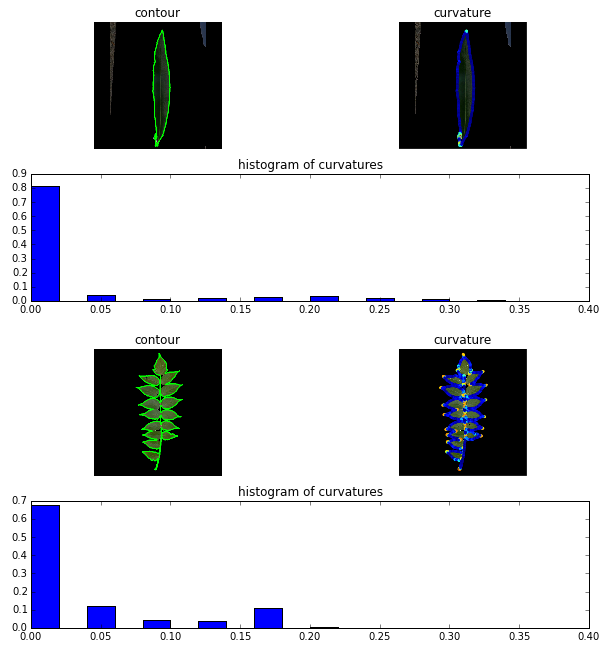
\includegraphics[width=0.6\linewidth]{img/curvatureHist.png}
  \caption{Histogrammes des courbures des images des feuilles 1 et 13}
  \label{curvaturehist}
\end{figure}


% Code integration example
%\begin{lstlisting}[language=bash]
%  sudo apt-get update
%  sudo apt-get install drupal7
%\end{lstlisting}

% Image integration example
%\begin{figure}[h]
%  \centering
%    \includegraphics[width=1\linewidth]{img/drupalFirstPage.png}
%  \caption{Page d'accueil du site créé avec Drupal sur une instance EC2}
%  \label{drupalfirstpage}
%\end{figure}
